\documentclass[11pt]{article}
\usepackage{fontspec}
\usepackage{ngerman}
\usepackage[top=3cm,left=3.5cm,right=3.5cm,bottom=3cm]{geometry}

\usepackage{amsmath}
\usepackage{listings}
\usepackage{graphicx}

\setromanfont{Charis SIL}
\setmonofont{Courier 10 Pitch}

\title{Control-Flow Integrity Checking}
\author{Hermann Loose}

\begin{document}

\maketitle

\section{Einführung}

% FIXME(hermannloose): Doofer Satzanfang.
Unerlaubter Kontrollfluss in Programmen stellt ein Problem sowohl für die
Sicherheit der Rechnersysteme auf denen diese Programme laufen als auch für die
Verlässlichkeit der von ihnen ausgeführten Berechnungen dar.

% Blah blah?
Es werden in der Folge zwei Verfahren betrachtet, die sich jeweils einem dieser
beiden Aspekte widmen und einander dabei in der Vorgehensweise zum Teil sehr
ähnlich sind.

\section{Control-Flow Integrity}

Das in \cite{abadi-2005-control-msr} vorgestellte Verfahren \emph{Control-Flow
Integrity} (CFI) zielt darauf ab, Angriffe zu verhindern, die auf dem Verlassen
des erlaubten Kontrollflusses in einem Programm aufbauen. Beispielhaft werden
stackbasierte Pufferüberläufe und darauf fußende Techniken, heapbasierte
\emph{jump-to-}\texttt{libc}-Angriffe sowie \emph{pointer subterfuge}-Angriffe
genannt.

Die Autoren argumentieren, dass viele der bisher gegen solche Angriffe
eingesetzten Mechanismen in ihrer Wirksamkeit beschränkt seien, da ihnen ein
realistisches Angreifermodell fehlen würde und sie sich selten auf formale
Schlüsse und häufig auf verborgene Annahmen stützten.

Die Antwort auf diese Probleme seien einfach verständliche Verfahren mit
dennoch umfassenden Garantien gegenüber starken Angreifern. Zudem sollten
praxistaugliche Techniken möglichst auf existierenden Code bzw. sogar auf
existierende Binärdateien anwendbar sein.

CFI als softwarebasierte Lösung wurde von den Autoren für Windows auf der x86
Architektur entwickelt und getestet; die Möglichkeit einer
Hardwareimplementierung von CFI wird hierbei kurz angesprochen, aber für die
nähere Zukunft als unwahrscheinlich bewertet. Ergänzend dazu wurde CFI in
\cite{abadi-2005-theory-fmse} für ein vereinfachtes Maschinenmodel
formalisiert.

\subsection{Grundlagen}

Das Angreifermodell für CFI beschreibt einen Angreifer, welcher „volle
Kontrolle über das Datensegment des ausführenden Programms besitzt“. Zusätzlich
wird die Möglichkeit zugelassen, dass der Angreifer bereits die Kontrolle über
ein anderes Modul oder einen anderen Thread im Adressraum besitzt. Als
tatsächliches Problem für die garantierte Einhaltung des erlaubten
Kontrollflusses identifizieren die Autoren daraufhin all die
Kontrollflusstransfers, deren Ziel im Programm erst zur Laufzeit bestimmt wird,
schließlich hat ein solcher Angreifer auf Transfers mit konstantem Ziel, wie
z.B. direkte Funktionsaufrufe, keinen Einfluss.

Um die Anwendung von CFI für existierende Software zu ermöglichen, wählten die
Autoren den Weg der Binärinstrumentierung von bereits übersetzten Programmen.
Durchgeführt wurde diese Instrumentierung mittels \emph{Vulcan}
\cite{edwards-vulcan}, von den Autoren als „reifes, state-of-the-art
Instrumentierungssystem für x86 Binärdateien“ beschrieben.

% TODO(hermannloose): Zur besseren Übersicht gerechtfertigt?
\subsubsection{Kontrollflussgraph}

Ausgangspunkt für das Verfahren ist ein \emph{Kontrollflussgraph} (CFG). Die
Knoten dieses Graphen bezeichnen sogenannte \emph{basic blocks}—Codeabschnitte
mit linearem Kontrollfluss ohne dynamische Transfers. Die gerichteten Kanten
des Graphen geben erlaubten Kontrollfluss zwischen diesen Knoten an.

Die erste Instruktion eines Knotens stellt ein erlaubtes Ziel für Transfers aus
den Startknoten der Eingangskanten dar. Am Ende des Knotens steht jeweils eine
Instruktion, welche ebenfalls den Kontrollfluss zur Laufzeit dynamisch bestimmt
und deren mögliche Ziele die Endknoten der ausgehenden Kanten sind.

% TODO(hermannloose): Holpriger Absatz, überarbeiten!
Mit Vorgriff auf die spätere Implementierung erfolgt zudem die Annahme, dass
Knoten, deren Eingangskanten gemeinsame Startknoten haben, äquivalente Ziele
darstellen, d.h. auf der Knotenmenge des Graphen ergeben sich
Äquivalenzklassen. Die Implikationen dieser Forderung werden später beleuchtet.
% FIXME(hermannloose): "Implikationen bezüglich was?" -> ausführen?

Die Autoren führen verschiedene Möglichkeiten für die Definition eines solchen
CFGs an, wobei sie sich für ihre Experimente auf CFGs konzentrieren, die durch
statische Analyse von Binärdateien gewonnen wurden, ebenfalls mittels Vulcan.

% TODO(hermannloose): An welcher Stelle Theorie einbauen?

\subsection{Instrumentierung}

Liegt ein solcher CFG vor, muss demnach zur Laufzeit vor Kontrollflusstransfers
mit dynamisch bestimmtem Ziel sichergestellt werden, dass vom aktuellen Knoten
zum jeweiligen Zielknoten eine Kante im CFG existiert.

Dazu wird jeder Äquivalenzklasse von Zielknoten im CFG eine ID zugewiesen und
direkt vor jedem Zielknoten im Codesegment eingefügt. Vor dem Transfer kann
daraufhin überprüft werden, ob die ID am aktuellen Ziel—dessen Adresse sich
z.B. in einem Register befindet—mit der ID der für diese Instruktion zulässigen
Ziele übereinstimmt.

Diese einleitende Betrachtung erfolgt unter Verwendung von erdachten
Instruktionen für Funktionsaufrufe und –rückkehr, welche jeweils die zulässige
Ziel-ID als Operand erhalten, sowie einer effektfreien Label-Instruktion, deren
Operand die ID des Knotens ist, welcher mit diesem Label versehen wird.

An dieser Stelle identifizieren die Autoren als Problem, dass mit dieser
Vorgehensweise nicht sichergestellt werden kann, dass Funktionen ausschließlich
zu ihrem jüngsten Aufrufort zurückkehren können. Es erfolgt der Verweis auf die
spätere Beschreibung eines auf CFI aufbauenden Verfahrens, welches diese
Beschränkung ermöglicht.

Die Autoren evaluieren in der Folge zwei konkrete Möglichkeiten der
Instrumentierung von Funktionsaufrufen.

\lstset{
  language=[x86masm]Assembler,
  basicstyle=\ttfamily\small,
  frame=lines
}

\begin{lstlisting}[title=Quelle]
  81 39 78 56 34 12  cmp  [ecx], 12345678h  ; comp ID & dst
  75 13              jne  error_label       ; if != fail
  8D 49 04           lea  ecx, [ecx+4]      ; skip ID at dst
  FF E1              jmp  ecx               ; jump to dst
\end{lstlisting}

\begin{lstlisting}[title=Ziel]
  78 56 34 12        ; data 12345678h       ; ID
  8B 44 24 04        mov  eax, [esp+4]      ; dst
  ...
\end{lstlisting}

Im ersten Fall stehen die Bytes der ID eines möglichen Ziels als Daten vor
diesem im Codesegment, Zieladressen von Kontrollflusstransfers zeigen jeweils
auf den Beginn dieser IDs. Der ID-Check an der Quelle vergleicht den Wert an
der Zieladresse mit einer als Immediate-Operand vorliegenden zulässigen ID.
% FIXME(hermannloose): Sehr holpriger Satz.
% FIXME(hermannloose): Eigentlich hier noch nicht konkret, da theoretische Betrachungen.
Schlägt dieser Vergleich fehl, erfolgt der Programmabbruch, mit einem von den
Autoren nicht weiter spezifizierten „Windows-Mechanismus zum Melden von
Sicherheitsverstößen“.

Als Problem wird bei dieser Methode angeführt, dass die Bytes der ID im
Codesegment sowohl am eigentlichen Ziel als auch in den Instruktionen des
ID-Checks vorkommen. Damit stellt die unmittelbar auf die Vergleichsoperation
folgende Instruktion—im Beispiel \texttt{jne error\_label}, zur
Fehlerbehandlung, was sich durch Präparieren der Prozessorflags umgehen
lässt—ein unerwartetes, gültiges Ziel dar.

\begin{lstlisting}[title=Quelle]
  B8 77 56 34 12     mov  eax, 12345677h    ; load ID-1
  40                 inc  eax               ; add 1 for ID
  39 41 04           cmp  [ecx+4], eax      ; compare w/ dst
  75 13              jne  error_label       ; if != fail
  FF E1              jmp  ecx               ; jump to label
\end{lstlisting}

\begin{lstlisting}[title=Ziel]
  3E 0F 18 05        prefetchnta            ; label
  78 56 34 12           [12345678h]         ;    ID
  8B 44 24 04        mov  eax, [esp+4]      ; dst
  ...
\end{lstlisting}

% TODO(hermannloose): Diese Variante wird von den Autoren später offensichtlich
% nicht verwendet.
Die zweite Herangehensweise löst diese Situation durch das Laden von ID–1 in
ein Register, nachfolgendes Inkrementieren und den Vergleich der ID am Ziel mit
dem enstandenden Wert.

\subsection{Annahmen}

Die Autoren setzen für den Einsatz von CFI drei Annahmen voraus:

\begin{description}

  \item [UNQ] \emph{Unique IDs:} „Nach der Instrumentierung dürfen die als IDs
  gewählten Bitmuster nirgendwo im Codesegment vorkommen außer in IDs und
  ID-Checks.“

  Die Autoren schlagen einen mindestens 32 Bit großen Schlüsselraum für die
  Wahl von IDs vor, um diese Annahme zu gewährleisten.

  \item [NWC] \emph{Non-Writable Code:} „Es darf dem Programm nicht möglich
  sein, das Codesegment zur Laufzeit zu verändern. Ansonsten wäre es einem
  Angreifer möglich, CFI z.B. durch das Überschreiben eines ID-Checks zu
  umgehen.“

  Während dies auf den meisten aktuellen Systemen gilt, weisen die Autoren auf
  problematische Fälle wie das Laden dynamisch gelinkter Bibliotheken und
  Codegenerierung zur Laufzeit hin.

  \item [NXD] \emph{Non-Executable Data:} „Es darf dem Programm nicht möglich
  sein, Daten als Code auszuführen. Ansonsten könnte ein Angreifer die
  Ausführung von Daten, welche mit der korrekten ID versehen sind, anstoßen.“

\end{description}

Es folgen einige Betrachtungen zum Verhalten des Systems, falls eine oder
mehrere Annahmen nicht gelten.

\subsection{Messungen}

Die in \cite{abadi-2009-control-tissec} diskutierten Messungen beziehen auf
bekannte Benchmarks aus dem SPEC-Paket. Sie wurden auf einem Pentium 4 x86 mit
1.8GHz und 512MB RAM unter Verwendung von Windows XP SP2 im \emph{Safe Mode},
bei dem ein Großteil der Dienste und Kernelmodule deaktiviert ist,
durchgeführt. Die untersuchten Programme wurden in Microsoft Visual C++ 7.1 mit
allen verfügbaren Optimierungen compiliert.

Die ermittelten Werte stellen jeweils den Durchschnitt von drei Durchläufen
dar, die Standardabweichung von weniger als einem Prozent wurde von den Autoren
als vernachlässigbar angesehen.

Der durchschnittliche Zuwachs an Größe für ein mit CFI instrumentiertes
Programm belief sich auf 8\%. Die Laufzeit der instrumentierten Programme stieg
um durchschnittlich 16\%. Die Autoren bewerten diesen Overhead als akzeptabel
und verweisen—ohne weitere Ausführungen—auf Möglichkeiten der Optimierung für
die x86 Implementierung von CFI.

% Kritik: wenig sicherheitsrelevante Ergebnisse, bereits 2004 im ersten Entwurf
% nur Sektion für Performancemessungen angelegt!

% FIXME(hermannloose): Besseren Titel finden.
\subsection{CFI als Grundlage für andere Verfahren}

% TODO(hermannloose): Zitate für IRMs und SMAC?
Aufgrund seiner Garantien für den Kontrollfluss von Programmen kann CFI zudem
als Grundlage für den Einsatz bzw. die Optimierung und Vereinfachung einer
Reihe anderer, ebenfalls softwarebasierter Mechanismen dienen. Die in
\cite{abadi-2009-control-tissec} beleuchteten sind \emph{Inlined Reference
Monitors} (IRMs) und \emph{Software Memory Access-Control} (SMAC).

% wie erkläre ich die zwei Verfahren, ohne hier einfach das Paper übersetzt zu
% reproduzieren? (oder ist das legitim?)

% FIXME(hermannloose): Anderen Titel finden.
% Ausblick nach sieben Jahren ist etwas müßig.
\subsection{Ausblick}

% Kritik: an dem Thema hat sich seit 2005 nichts getan
\cite{abadi-2009-control-tissec} erschien zuerst im Februar 2005 als Technical
Report von Microsoft Research \cite{abadi-2005-control-msr}. Spätere
Veröffentlichungen 2005 und 2007 sind inhaltlich identisch. Zum Problem des
Umgangs mit selbstmodifizierendem Code und Codegenerierung zur Laufzeit erfolgt
in \cite{abadi-2005-control-msr} der Verweis „we are working on […] handling
runtime code generation and other dynamic additions of code“, seit 2007 und in
\cite{abadi-2009-control-tissec} lautet diese Stelle nunmehr „we have
considered working on […] handling runtime code generation and other dynamic
additions of code“, was nahelegt, dass hier kein weiterer Fortschritt erfolgt
ist. % TODO(hermannloose): Zitate checken.

% beleuchten: ist Overhead ein Problem?

\section{Control-Flow~Checking by Software~Signatures}

% Grundsätzlich fertig.

Im Gegensatz zu CFI beschäftigt sich das 2002 in \cite{oh-2002-control}
beschriebene Verfahren \emph{Control-Flow Checking by Software Signatures}
(CFCSS) mit der Erkennung von unerlaubtem Kontrollfluss, nachdem dieser bereits
aufgetreten ist. Das Augenmerk liegt dabei auf transienten oder permanenten
Hardwarefehlern als Auslöser. Die Autoren identifizieren dadurch in der Folge
unentdeckt bleibende, da nicht von Programmabstürzen begleitete Verfälschungen
von Ergebnissen als Hauptproblem.

Der Ausgangspunkt ist wie bei CFI eine softwarebasierte Lösung. Als Motivation
wird das Stanford \emph{Advanced Research and Global Observation Satellite}
(ARGOS) Projekt angeführt. Das auf diesem Satelliten befindliche
\emph{Unconventional Stellar Aspect} (USA)
Experiment\footnote{http://xweb.nrl.navy.mil/usa/publications/usa-xrb.html}
trug neben einem strahlungsfesten RH-3000 Single-Board-Computer mit
verschiedenen Möglichkeiten zur Erkennung und Korrektur von Hardwarefehlern ein
äquivalentes Board aus herkömmlichen Komponenten zum
Vergleich \cite{argos-2002-lessons}. Für letzteres beschränkten sich
Fehlererkennung und –behebung auf Softwaremethoden, einschließlich CFCSS.

% Grundsätzlich alles enthalten, muss aber noch zum Ende hin überarbeitet werden.
\subsection{Konzept}

CFCSS stützt sich wie CFI auf einen Kontrollflussgraphen, dessen Kanten
erlaubten Kontrollfluss in einem Programm aufzeigen. Im Unterschied zu CFI
erhält hier allerdings jeder Knoten $v_i$ seine eigene Signatur $s_i$. Ein vom
Compiler oder Assembler ausgewähltes Register dient als \emph{Global Signature
Register} (GSR), welches zur Laufzeit jeweils die Signatur des aktuellen
Knotens enthalten sollte. Ist dies nicht der Fall, liegt fehlerhafter
Kontrollfluss vor.

% FIXME(hermannloose): Holprig, verbose.
Es folgt zunächst die Betrachtung für den Fall einer einzelnen eingehenden
Kante in einen Knoten. Der neue Inhalt des GSRs wird beim Eintritt in den
Knoten durch eine Signaturfunktion $f$ aus der aktuellen Signatur $G$ im
Register und einem die Kante eindeutig auszeichnenden Wert $d_i$ berechnet.

% TODO(hermannloose): Sollte die Wahl von XOR evtl einfacher abgespeist werden?
Hierfür wählten die Autoren die XOR-Verknüpfung der Signatur des Startknotens
der Kante $s_s$ und der Signatur des Endknotens $s_d$, d.h. $d_d \equiv s_s
\oplus s_d$. Die Signaturfunktion ergibt sich dann zur Laufzeit als $f \equiv
f(G, d_i) = G \oplus d_i$.

Die Autoren motivieren die Wahl von XOR damit, dass die Operationen AND, OR und
XOR in der ALU aus weniger Gattern bestehen und somit die Wahrscheinlichkeit
eines transienten Hardwarefehlers während der Berechnung der neuen Signatur
geringer ausfällt. Aus dieser Menge ist nur für XOR bei einem gegebenen
Operanden und bekanntem Ergebnis der andere Operand eindeutig bestimmt, was zur
sicheren Erkennung von ungültigem Kontrollfluss notwendig ist.

% TODO(hermannloose): Die Beispiele sind ziemlich verbose und können evtl raus.
Enthält das GSR nun z.B. im Knoten $ v_1 $ die Laufzeitsignatur $ G_1 = s_1 $ und
es erfolgt ein erlaubter Transfer zum Knoten $ v_2 $, so berechnet sich die neue
Laufzeitsignatur $ G_2 $ wie folgt: $$ G_2 = f(G_1, d_2) = G_1 \oplus d_2 = s_1
\oplus (s_1 \oplus s_2) = s_2 $$

Erfolgt stattdessen ein unerlaubter Transfer von $ v_1 $ zu $ v_4 $, wobei
$ v_4 $ für erlaubte Transfers von $ v_3 $ ein $ d_4 = s_3 \oplus s_4
$ enthält, berechnet sich die neue Laufzeitsignatur als $$ G_4 = f(G_1, d_4)
= G_1 \oplus d_4 = s_1 \oplus (s_3 \oplus s_4) \neq s_4 $$ und im Knoten $v_4$
wird ein Fehler im Kontrollfluss erkannt.

% TODO(hermannloose): Beispiel mit Sprung in die Mitte eines Blocks auch explizit?

Damit ergibt sich allerdings ein Problem im Fall eines sogenannten
\mbox{\emph{branch fan-in}} Knotens mit mehreren Eingangskanten. Ist im
Beispiel von Abbildung~\ref{fig:fanin-node} $ d_5 = s_1 \oplus s_5 $, schlägt
ein eigentlich gültiger Transfer von $ v_3 $ nach $ v_5 $ nach dem bisherigen
Verfahren fehl. Es ist allerdings auch nicht möglich, einfach $ s_1 = s_3 $ zu
setzen, weil damit ungültige Transfers von $ v_1 $ nach $ v_4 $ und $ v_3
$ nach $ v_2 $ nicht mehr erkannt würden.

\begin{figure}
  \centering
  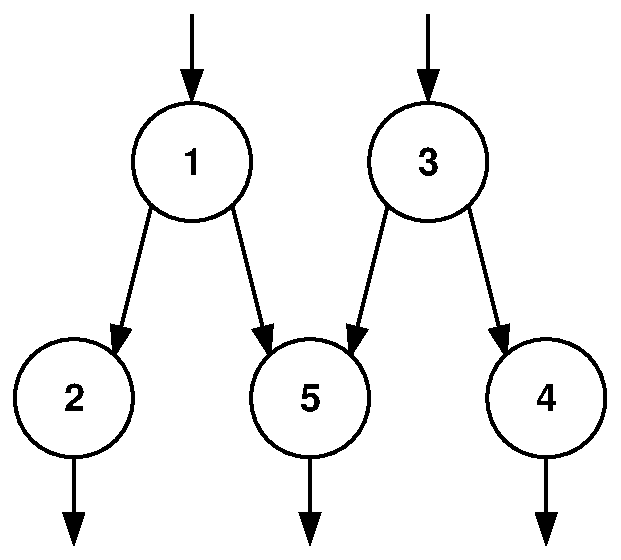
\includegraphics[width=0.5\textwidth]{fanin-node}
  \caption{Beispiel für \emph{branch fan-in} Knoten}
  \label{fig:fanin-node}
\end{figure}

Um diese Situation zu beheben führen die Autoren einen zusätzlichen Wert
$ D $ ein. Dieser wird vor dem Transfer im Startknoten gesetzt und im
Zielknoten mit der berechneten Laufzeitsignatur $ G $ XOR-verknüft.  Wurde
$ d_d $ im Zielknoten $ v_d $ als $ s_s \oplus s_d $ für einen Startknoten
$ v_s $ bestimmt, wird $ D $ in $ v_s $ auf $ 0 $ gesetzt. Für alle anderen
Startknoten $ v_i $ ergibt sich $ D $ als $ s_i \oplus s_s $.

Erfolgt im Beispiel der Transfer von $ v_1 $ nach $ v_5 $ so gilt $$ G_5
= f(G_1, d_5) \oplus D = s_1 \oplus (s_1 \oplus s_5) \oplus 0 = s_5 $$

Für den Transfer von $ v_3 $ nach $ v_5 $ gilt $$ G_5 = f(G_3, d_5) \oplus
D = s_3 \oplus (s_1 \oplus s_5) \oplus (s_3 \oplus s_1) = s_5 $$

% TODO(hermannloose): "Algorithmus" genau beschreiben?
Die Autoren geben einen einfachen Algorithmus an, um anhand eines vorliegenden
CFGs das genannte Vorgehen zur Compilezeit zu realisieren.

Es folgen Betrachtungen der Autoren zur Erkennbarkeit von ungültigen
Kontrollflusstransfers. Zusammengefasst sagen diese aus, dass unerlaubte
Verzweigungen zu einem Knoten erkannt werden, ungeachtet dessen welche
Instruktion in diesem Knoten getroffen wird. Ebenso erfasst das Verfahren das
Entfernen von unbedingten Verzweigungen am Ende eines Knotens, da dieser mit
seinem Nachfolger im Code verschmilzt und die Signaturfunktion des
Nachfolgerknotens eine ungültige Laufzeitsignatur generiert.

Als weiteres Korollar wird angeführt, dass das Einfügen einer
Verzweigungsinstruktion in einen Knoten erkannt wird, solange diese Verzweigung
auf Knotenebene keine erlaubte ist. An dieser Stelle gehen die Autoren nicht
weiter auf den Fall ein, dass eine Verzweigung eingefügt wird, welche laut CFG
gültig ist—diese Gültigkeit bezieht sich jedoch implizit nur auf die
Instruktion am Ende des Basic Blocks. In dieser Situation würden Instruktionen
im Knoten welche nach der eingefügten Verzweigung folgen übersprungen, ohne
dass fehlerhafter Kontrollfluss feststellbar wäre.

Da bei den im folgenden Abschnitt angegebenen Messungen trotz des Einsatzes von
CFCSS ein geringer Prozentsatz von unentdeckt verfälschten Programmergebnissen
sichtbar wird, scheint das genannte Problem tatsächlich eine Fehlerquelle
darzustellen.

% Grundsätzlich fertig, kaum Eigenanteil.
\subsection{Messungen}

In \cite{oh-2002-control} finden sich zu CFCSS nur Simulationsergebnisse, wobei
dieses Paper in \cite{argos-2002-lessons} zitiert wird, also zu einem
Zeitpunkt, als bereits Messwerte vom Einsatz auf dem Satelliten vorlagen.

Die Autoren wählten sieben Benchmarks für ihre Experimente aus:

\begin{itemize}
  \item LZW-Kompression
  \item FFT
  \item Matrixmultiplikation
  \item Quicksort
  \item Insertsort
  \item Türme von Hanoi
  % TODO(hermannloose): Siehe Notiz.
  \item Shuffle – \emph{nicht weiter spezifiziert, was darunter zu verstehen ist}
\end{itemize}

Die zugehörigen Quelltexte wurden zunächst ohne CFCSS für die MIPS-Architektur
kompiliert. Daraufhin wurde einer der im Folgenden beschriebenen Fehler
zufällig in den entstandenen Assembler-Code eingefügt:

\begin{itemize}
  \item eine Verzweigungsinstruktion wurde durch ein NOP ersetzt,
        d.h. zwei im Quelltext aufeinander folgende Knoten des Kontrollflussgraphen
        verschmelzen zu einem einzelnen
  % FIXME(hermannloose): Holprig.
  \item eine unbedingte Verzweigungsinstruktion wurde zufällig im Programm eingefügt
  \item der Immediate-Operand einer Verzweigungsinstruktion wurde verändert
\end{itemize}

% FIXME(hermannloose): Holprig.
Der fertig assemblierte Binärcode wurde schließlich auf einer SGI Indigo mit
R4400 MIPS-Prozessor ausgeführt, die in \cite{oh-2002-control} beschriebenen
Ergebnisse beziehen sich auf jeweils 500 Iterationen der Benchmarks. Für die
Auswertung wurden die auftretenden Fehler ob ihrer Natur und Erkennbarkeit
unterteilt, so z.B. Endlosschleifen, Fehler die keine Auswirkungen auf das
Ergebnis einer Berechnung hatte, Fehler, die vom Betriebssystem in Form von
Abstürzen—z.B. Speicherzugriffsverletzungen und fehlschlagende
Assertions—erkannt wurden etc.; hierbei lag der Fokus auf Fehlern, die
unentdeckt Programmergebnisse verfälschten, was im Durchschnitt bei 33,7\% der
eingefügten Fehler der Fall war.

Im zweiten Durchgang wurden die Benchmarks zusätzlich zu den eingefügten
Fehlern auf Assemblerebene mit CFCSS ausgestattet. In der Folge erzeugten nur
noch 3,1\% dieser Fehler unentdeckt verfälschte Programmergebnisse.

Die Autoren führen weiterhin Daten zum Overhead bei Größe und Ausführungszeit
an, im Kontext der Gesamtzahl von Instruktionen jedes Benchmarks, Anzahl der
eingefügten Instruktionen des Checking-Codes sowie der durchschnittlichen Länge
der Basic Blocks. Für die Programmgröße beträgt der Overhead durchschnittlich
45,2\%, für die Ausführungszeit 43,1\%.

Es wird hierbei kurz bemerkt, dass rechenintensive Anwendungen ohne häufige
Verzweigungen (im Beispiel FFT) grundsätzlich längere Basic Blocks haben und
Overhead daher besonders bei Such- und Sortieralgorithmen mit sehr kurzen Basic
Blocks und ständigen Verzweigungen zum Tragen kommt.

% TODO(hermannloose):
% evtl. Zahlen aus "Lessons Learned"? Falls sich dort was spezifisches zu CFCSS
% finden lässt, kann sein, das ist nicht weiter von EDDI (dem anderen
% Verfahren) getrennt
% -> dort findet sich nicht viel zum Verhältnis, aber geringe Zahlen zu von
%  CFCSS erkannten Fehlerzuständen

% Grundsätzlich fertig, kaum Eigenanteil.
\subsection{Optimierung}

% FIXME(hermannloose): Evtl kann der Absatz auch einfach raus. Ist sowieso mehr
% oder weniger abgepinselt.
Je nach Architektur benötigt die Berechnung einer neuen Laufzeitsignatur und
der nachfolgende Vergleich mit der erwarteten Signatur etwa zwei bis vier
Instruktionen. Bei einer durchschnittlichen Länge eines Basic Blocks von z.B.
sieben bis acht Instruktionen beträgt der Overhead für die Programmgröße
zwischen 25\% und 43\%. % FIXME(hermannloose): Ich komme hier auf 20% bis 36%??

Falls Fehler nicht sofort behandelt werden müssen, kann an dieser Stelle auf
den Vergleich der Signaturen und die folgende Verzweigung verzichtet werden.
Solange die Laufzeitsignatur korrekt aktualisiert wird, lässt sich zu jedem
späteren Zeitpunkt feststellen, dass im Kontrollfluss Fehler vorgelegen haben.
Der Overhead des Verfahrens lässt sich somit auf Kosten späterer
Fehlererkennung reduzieren.

Als ein mögliches Vorgehen in der Praxis schlagen die Autoren im Beispiel vor,
statt in jeder Iteration einer Schleife nur am Ende dieser die Signaturen zu
vergleichen, oder für sich auf höherer Ebene verzweigenden Code den
Signaturvergleich auf den Zeitpunkt zu verschieben, an dem sich mehrere
Verarbeitungszweige wieder vereinen. Die quantitativen Betrachtungen hierzu
bleiben theoretischer Natur.

\pagebreak
\bibliographystyle{unsrt}
\bibliography{paper}

\end{document}
